% TrustNav: IEEE conference-style paper.
% Build:  cd paper && pdflatex trustnav.tex && pdflatex trustnav.tex
% (IEEEtran.cls is shipped alongside; on Overleaf, upload the whole folder.)
\documentclass[conference]{IEEEtran}
\IEEEoverridecommandlockouts
\usepackage[utf8]{inputenc}
\usepackage[T1]{fontenc}
\usepackage{cite}
\usepackage{amsmath,amssymb}
\usepackage{graphicx}
\usepackage{booktabs}
\usepackage{array}
\usepackage{xurl}
\usepackage{xcolor}
\usepackage{tikz}
\usetikzlibrary{arrows.meta,positioning,shapes.misc}
\usepackage{balance}
\usepackage[hidelinks]{hyperref}
\def\BibTeX{{\rm B\kern-.05em{\sc i\kern-.025em b}\kern-.08em T\kern-.1667em\lower.7ex\hbox{E}\kern-.125emX}}
\newcommand{\sys}{TrustNav}

\begin{document}

\title{\sys: Explainable Per-Second Trust Scoring and Response for GNSS Spoofing and Jamming in Vehicle and Drone Fleets}

\author{
\IEEEauthorblockN{Karan Deshmukh, Niranjan Satheesh Thandassery, Sudheer Reddy Jogi, Venkata Pavan Kumar Sanam}
\IEEEauthorblockA{MSc Cybersecurity and Data Science, ESAIP \'Ecole d'Ing\'enieurs, Angers, France\\
Group 2, technical project supervised by Sofiane Hamrioui\\
Corresponding author: domail2karandeshmukh@gmail.com}
}

\maketitle

\begin{abstract}
Fleet software believes the satellite position its receivers report. Jamming (drowning the signal) and spoofing (feeding a false position) are now daily events in parts of Europe and require only inexpensive equipment, yet existing countermeasures either live inside a single receiver and emit an unexplained flag, or monitor a fixed site. We present \sys, a software system that scores, once per second and for every vehicle and drone in a fleet, how much its reported position can be believed (0--100), explains the score in plain words, and \emph{responds}: a position below the trust line is refused and replaced downstream by an estimate dead-reckoned from the odometer along the planned route. Three kinds of evidence are fused by noisy-OR: fifteen physical and signal rules with named thresholds, an unsupervised anomaly model (Isolation Forest and a per-feature tail detector) trained on normal driving only, and Galileo Open Service Navigation Message Authentication (OSNMA). On ten held-out scenarios produced by a deterministic simulator over real Angers street geometry (3\,800 one-second observations), the combined detector reaches 99.3\,\% precision, 96.1\,\% recall and a 0.44\,\% false-alarm rate, catches all seven attack types, and detects a relay-style ``stealth'' drift that passes OSNMA after 42\,s where a fixed 150\,m rule would need about 3.5\,min. The response layer bounds the worst operator-visible position error from 8.0\,km to 29\,m and removes the 100\,s blank screen caused by jamming. The complete system (engine, cloud back end, live console, receiver adapter) is open source; its limits, chiefly that all data are synthetic, and the plan to validate it on a real receiver are discussed.
\end{abstract}

\begin{IEEEkeywords}
GNSS, spoofing, jamming, Galileo OSNMA, anomaly detection, Isolation Forest, explainable AI, fleet telematics, dead reckoning, cybersecurity.
\end{IEEEkeywords}

\section{Introduction}
Almost everything that moves relies on a Global Navigation Satellite System (GNSS) position and trusts it without question: delivery vans, trucks, taxis, emergency vehicles, trams, ships, agricultural machines and drones. That trust is easy to break. GNSS signals reach the ground about 20\,000\,km from the satellite and are extremely weak, so a small transmitter nearby can either drown them (\emph{jamming}) or imitate them and feed the receiver a false but believable position (\emph{spoofing}). Jammers costing tens of euros are sold illegally and are regularly found in vehicles whose drivers want to escape fleet tracking \cite{anfr2024}; one left running in a car parked at Nantes airport delayed flights in 2017 \cite{rntf2017}, another disrupted a GNSS landing aid at Lyon airport in 2023 \cite{transinfo2023}, and a jammer in a contractor's pickup truck interfered with the ground-based augmentation system under test at Newark airport \cite{insidegnss2013}. Since 2022, interference around the Baltic Sea and the Middle East has grown into a daily event for aviation, with about 1\,500 flights spoofed per day by the summer of 2024 \cite{eucouncil2025,opsgroup2024}.

Two gaps motivate this work. First, the fleet telematics platforms that operators actually use display the reported position and, at most, relay the receiver's own jamming flag \cite{geotab2025}; they do not say whether the position is true. Second, the detection products that exist either run inside one receiver and output a state code with no explanation \cite{ublox2024,septentrio2025}, or are fixed multi-antenna probes that protect a site rather than a moving platform \cite{gpspatron}. We argue that the natural place for a defence is a software layer beside the receiver, working on what any receiver already reports, that (i) gives each platform a per-second trust score, (ii) explains it in terms an operator can verify, and (iii) acts on it so that nothing downstream consumes a lie.

\sys\ implements this layer. Our contributions are:
\begin{enumerate}
\item a hybrid detector that fuses fifteen explainable physical and signal rules, an unsupervised anomaly model trained on normal operation only, and Galileo OSNMA status, with a calibrated mapping from anomaly probability to risk so that the alert line has a stated meaning;
\item a \emph{response layer} that refuses untrusted fixes and substitutes a route-constrained dead-reckoned estimate from the odometer, with a rejoin rule that a spoofer cannot defeat by briefly looking clean;
\item a complete, open-source implementation: a Python engine, a cloud back end with authenticated ingest, a live console that explains every decision in plain words, and an adapter for real receivers;
\item an evaluation protocol with disjoint training, validation and held-out routes on real Angers street geometry, and a quantified measure of what the response layer prevents.
\end{enumerate}

Section~\ref{sec:related} reviews existing countermeasures. Section~\ref{sec:design} describes the detector and the response layer, Section~\ref{sec:impl} the implementation, Section~\ref{sec:eval} the evaluation and results, Section~\ref{sec:discussion} the limitations and the road to a real receiver, and Section~\ref{sec:ethics} the safety and legal frame.

\section{Background and Related Work}\label{sec:related}

\subsection{Threats}
A \emph{jammer} transmits noise in the GNSS bands; the receiver's carrier-to-noise density ratio (C/N$_0$) collapses, satellites are lost and eventually no position fix is computed. A \emph{spoofer} transmits counterfeit satellite signals; a simple spoofer captures the receiver and moves the fix abruptly (``teleport''), a careful one pulls it away slowly (``drift''). A \emph{relay} or meaconing attack re-broadcasts genuine signals with a delay, so the navigation data remain authentic while the position is wrong. \emph{Forgery} fabricates navigation messages themselves. Each leaves different traces in the receiver's observables: motion that is physically impossible, signals that are stronger and more uniform than real satellites, range residuals that disagree, clock behaviour that jumps, or authentication that fails.

\subsection{Galileo OSNMA}
Galileo's Open Service Navigation Message Authentication signs the I/NAV navigation data with a TESLA delayed-disclosure scheme and was declared operational on 24 July 2025 \cite{euspa2025}; it is mandatory in smart tachographs for new EU trucks and buses from December 2025. OSNMA lets a receiver flag unauthenticated data, but the EU GNSS Service Centre states that it gives no protection against jamming and does not by itself prevent spoofing \cite{gsc_faq}; GPS data are not covered, and replay attacks that pass OSNMA have been demonstrated on real receivers \cite{wang2025}. OSNMA is therefore one kind of evidence, not a complete defence.

\subsection{Receiver-level detection}
Mass-market u-blox receivers report a spoofing state (unknown, none, indicated, multiple indications) and a jamming state; recent firmware adds a jamming log, OSNMA and per-band flags \cite{ublox2024}. The vendor notes that a ``no spoofing'' state does not prove the absence of spoofing, that detection requires first locking to genuine signals, and at the Jammertest 2025 campaign both flags tripped during a jamming-only run \cite{ublox_jammertest}. Septentrio's AIM+ combines notch filters, a spectrum view and spoofing and meaconing flags inside its receivers \cite{septentrio2025}. These mechanisms are per receiver and binary; \sys\ consumes them as inputs rather than competing with them.

\subsection{Fixed probes and anti-jamming hardware}
GPSPatron operates rack-mounted probes with up to three antennas that stream raw observables to a cloud which classifies jamming and spoofing types; the three-antenna probe needs at least 1\,m of antenna separation \cite{gpspatron}. infiniDome's GPSdome null-steers jammers with two or more antennas placed between antenna and receiver \cite{gpsdome2}. Both protect a place or require extra hardware on every vehicle; neither explains its decision to a fleet operator.

\subsection{Fleet telematics}
Geotab's newer GO devices log a jamming event (named \texttt{GpsJammingDetected}) that the GPS module's own detector raises \cite{geotab2025}; we found no spoofing detection claim from Geotab and nothing on jamming or spoofing from Samsara or Webfleet. Aviation interference maps derived from ADS-B integrity fields \cite{gpsjam,fr24} show \emph{where} interference occurs at country scale with a six- to twenty-four-hour refresh and cannot separate jamming from spoofing.

\subsection{Machine-learning detection}
Recent work applies learned models to receiver observables, mostly on the TEXBAT recordings \cite{texbat}: an LSTM-based network with a conditional VAE reaches an F1 of 96.9\,\% \cite{tang2025}; a convolutional VAE trained on clean data only reaches near-perfect true-positive rates on the easier sets and 89\,\% on the hardest \cite{iqbal2025}; a random forest on multi-parameter features exceeds 97\,\% \cite{li2025}; a chi-square test on raw intermediate-frequency samples reports over 99\,\% accuracy with no false alarms on public recordings and a jammer test campaign \cite{bhuiyan2026}. Closest to our setting, Kriezis \emph{et al.} evaluated rule-based checks on a \texteuro200 u-blox ZED-F9P against real spoofing in the eastern Mediterranean: C/N$_0$, residuals and clock drift were informative, automatic gain control and Doppler were not, and the aviation MOPS interference algorithm scored 94\,\% on one receiver but below 13\,\% on another \cite{kriezis2025}. That receiver dependence shapes our validation plan (Section~\ref{sec:discussion}). \sys\ belongs to the same family but is a \emph{system}: it adds the route and the odometer as evidence a receiver cannot supply, reports per-second trust rather than a binary verdict, explains each decision, and responds.

\section{System Design}\label{sec:design}

\begin{figure}[t]
\centering
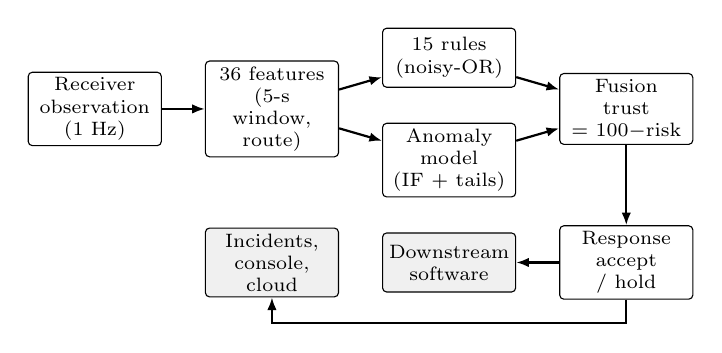
\begin{tikzpicture}[font=\scriptsize, x=1cm, y=1cm,
  box/.style={draw, rounded corners=1.5pt, align=center, inner sep=2pt, minimum height=7.5mm, text width=1.55cm},
  sink/.style={box, fill=black!6},
  arr/.style={-{Latex[length=1.6mm]}, thick}]
\node[box] (obs) at (0,0) {Receiver\\observation (1 Hz)};
\node[box] (feat) at (2.25,0) {36 features\\(5-s window, route)};
\node[box] (rules) at (4.5,0.65) {15 rules\\(noisy-OR)};
\node[box] (model) at (4.5,-0.65) {Anomaly model\\(IF + tails)};
\node[box] (fuse) at (6.75,0) {Fusion\\trust $=100-$risk};
\node[box] (resp) at (6.75,-1.95) {Response\\accept / hold};
\node[sink] (down) at (4.5,-1.95) {Downstream\\software};
\node[sink] (inc) at (2.25,-1.95) {Incidents, console,\\cloud};
\draw[arr] (obs) -- (feat);
\draw[arr] (feat) -- (rules);
\draw[arr] (feat) -- (model);
\draw[arr] (rules) -- (fuse);
\draw[arr] (model) -- (fuse);
\draw[arr] (fuse) -- (resp);
\draw[arr] (resp) -- (down);
\draw[arr] (resp.south) -- ++(0,-0.3) -| (inc.south);
\end{tikzpicture}
\caption{Processing pipeline. Every observation (position, speed, signal statistics, clock, OSNMA status, odometer speed) becomes a feature vector, is judged by rules and by an anomaly model, fused into a trust score with evidence, and passed to the response layer, which decides which position downstream software receives.}
\label{fig:pipeline}
\end{figure}

\subsection{Observations and features}
Once per second the receiver reports position, speed, heading, satellites tracked, C/N$_0$ statistics, position dilution of precision (PDOP), pseudorange residuals, clock bias and drift, a jamming indicator, OSNMA status and, where available, an inertial or odometer speed. A single reading says little; what matters is how it compares with the previous seconds and with the route the platform is expected to follow. A streaming feature extractor keeps a rolling window of five observations and computes 36 features, among them the distance moved since the last fix, derived versus reported speed, acceleration and heading rate, distance to the assigned route, C/N$_0$ mean, change and spread, satellite-count change, PDOP, residuals, clock deltas, the GNSS-versus-inertial speed mismatch, and explicit \texttt{missing\_*} flags so that an absent input is never mistaken for zero. The extractor is incremental, so the same code scores recorded data and live data.

\subsection{Rules}
Fifteen deterministic checks compare a feature with a named threshold drawn from the platform's physical profile (for a road vehicle: 60\,m/s, 8\,m/s$^2$, 90$^\circ$/s, 250\,m per second) or from signal physics (a 6\,dB-Hz C/N$_0$ shift, PDOP above 5, residuals above 12\,m, a clock-drift change above 60\,ns/s, a jamming indicator above 80/255, satellite changes of five or more), plus OSNMA failed or lost and fix lost. A rule's contribution $c_i$ is its weight times a severity that rises from 0.5 at the threshold to 1.0 at three times the threshold; rules combine by noisy-OR,
\begin{equation}
r_{\mathrm{rules}} = 100\,\Bigl(1-\prod\nolimits_i (1-c_i)\Bigr),
\end{equation}
so that independent evidence reinforces itself. Two conditions are \emph{critical}: a position jump above four times the profile limit and an OSNMA failure; either pins the combined risk at 70 or more. Thresholds sit where behaviour becomes physically implausible, not where an attack becomes likely, which keeps the rules almost silent on normal data at the cost of missing slow attacks.

\subsection{Anomaly model}
Because any supervised model would learn the shapes of the simulator's attacks, the learned component is trained on \emph{normal operation only}. Two detectors complement each other: an Isolation Forest \cite{liu2008} (300 trees, scikit-learn \cite{sklearn}) finds unusual combinations of the 19 model inputs, and a per-feature tail detector finds a single improbable input, such as a fix 90\,m off the road while every signal statistic is clean, and names it. Each detector's raw score is converted to a tail probability $p$ on a calibration set of normal runs not used for fitting (the fraction of normal observations at least as anomalous), the two are combined with a Bonferroni correction, $p=\min(1,\,2\min(p_{\mathrm{forest}},p_{\mathrm{tail}}))$, and the risk is
\begin{equation}
r_{\mathrm{model}} = 100\,\min\!\left(1,\ \frac{-\log_{10} p}{4}\right),
\end{equation}
so a risk of 50 corresponds to roughly a one-in-a-hundred event under normal operation. A plain percentile rank would spread normal data uniformly over 0--100 and make a risk-50 alert fire on half of all clean seconds. A trailing median over three seconds suppresses isolated spikes while sustained anomalies survive. When the risk is 25 or more the model explains itself by listing its most unusual inputs with their normal ranges.

\subsection{Fusion, trust and incidents}
Rules and model are two witnesses, not two votes to average: a confident model alarm of 90 averaged with quiet rules at 20 would give 55, weaker than the model alone. The combined risk is a weighted noisy-OR,
\begin{equation}
r = 100\,\bigl(1-(1-w_r\,p_r)(1-w_m\,p_m)\bigr),\qquad \mathrm{trust}=100-r,
\end{equation}
with $p_r=r_{\mathrm{rules}}/100$ and $p_m=r_{\mathrm{model}}/100$. The weights $w_r=0.6$ and $w_m=0.8$ were chosen by grid search on validation routes only. Trust bands are Trusted ($\ge75$), Degraded (50--74), Suspicious (25--49) and Untrusted ($<25$). An incident opens after three consecutive seconds below 50 and closes after five clean seconds; its title names the strongest critical evidence.

\subsection{Response layer}
Detection alone leaves the operator looking at a lie. The response layer turns the score into an action, in the way an intrusion prevention system acts on what an intrusion detection system finds. A fix is \emph{accepted} when it is present, its trust is at least 50 and no critical rule fired. Otherwise it is \emph{held}: the fix is refused, and the position handed downstream is dead-reckoned from the last accepted fix using the odometer speed, which a spoofer cannot touch. With an assigned route the estimate advances along the route (map-matched), so the lateral error of the last accepted fix is dropped and only along-track odometer error accumulates; without a route it continues on the last accepted heading. Where a route doubles back on itself, projection onto the route uses the direction of travel and continuity with the previous arc-length position to pick the right leg. A hold is \emph{released} only after five consecutive acceptable observations whose fix lies within 60\,m plus 3\,\% of the distance dead-reckoned while held, so a spoofer cannot end the hold by looking clean while still far away; a sixty-second clean streak releases regardless, with the discrepancy reported, because an odometer estimate drifts too. Each observation also carries a recommended action: \textsc{continue}, \textsc{verify} (confirm by other means before acting) or \textsc{isolate} (trust below 25 or critical evidence: stop using the device's position; a drone holds or returns on inertial navigation, a driver is contacted).

\section{Implementation}\label{sec:impl}
\sys\ is open source\footnote{\url{https://github.com/domail2karandeshmukh-cyber/trustnav}} and deployed as a public demonstration.\footnote{\url{https://trustnav.vercel.app}} The \textbf{engine} is Python (NumPy, scikit-learn): a deterministic simulator, the feature extractor, rules, model, fusion, incident tracker, response layer, evaluation and a live streamer; 23 automated tests cover its behaviour, including that noisy-OR is stronger than either witness, that a critical rule pins the floor, that holds do not release while the returning fix is still far away, and that the route odometer tracks a jammed vehicle within 2\,m over a minute. A \textbf{receiver adapter} parses NMEA sentences (GGA, RMC, VTG, GSA, GSV) and u-blox UBX messages (NAV-PVT, NAV-CLOCK, NAV-STATUS, NAV-SAT, MON-HW) from a serial port or a log into the same observation dictionary, so a real receiver plugs into the same detector; it is tested on synthetic streams. The \textbf{cloud} side is Supabase (PostgreSQL with row-level security, realtime channels, a scheduled demo feed): the browser can only read; writes pass through an edge function that checks a token stored as a SHA-256 hash; presenter actions sit behind a bcrypt-hashed passcode with rate limiting; secrets are never in the repository. The \textbf{console} is a Next.js application with a MapLibre street map of Angers (OpenStreetMap data, 3D buildings), a live fleet view, replay of ten recorded scenarios with a narrated story, a space--time view, a presentation mode, a narrated explainer in ten languages, and an operator playbook; 98 end-to-end checks (Playwright, including an accessibility scan) run on every build. Fig.~\ref{fig:console} shows the deployed console.

\begin{figure}[t]
\centering
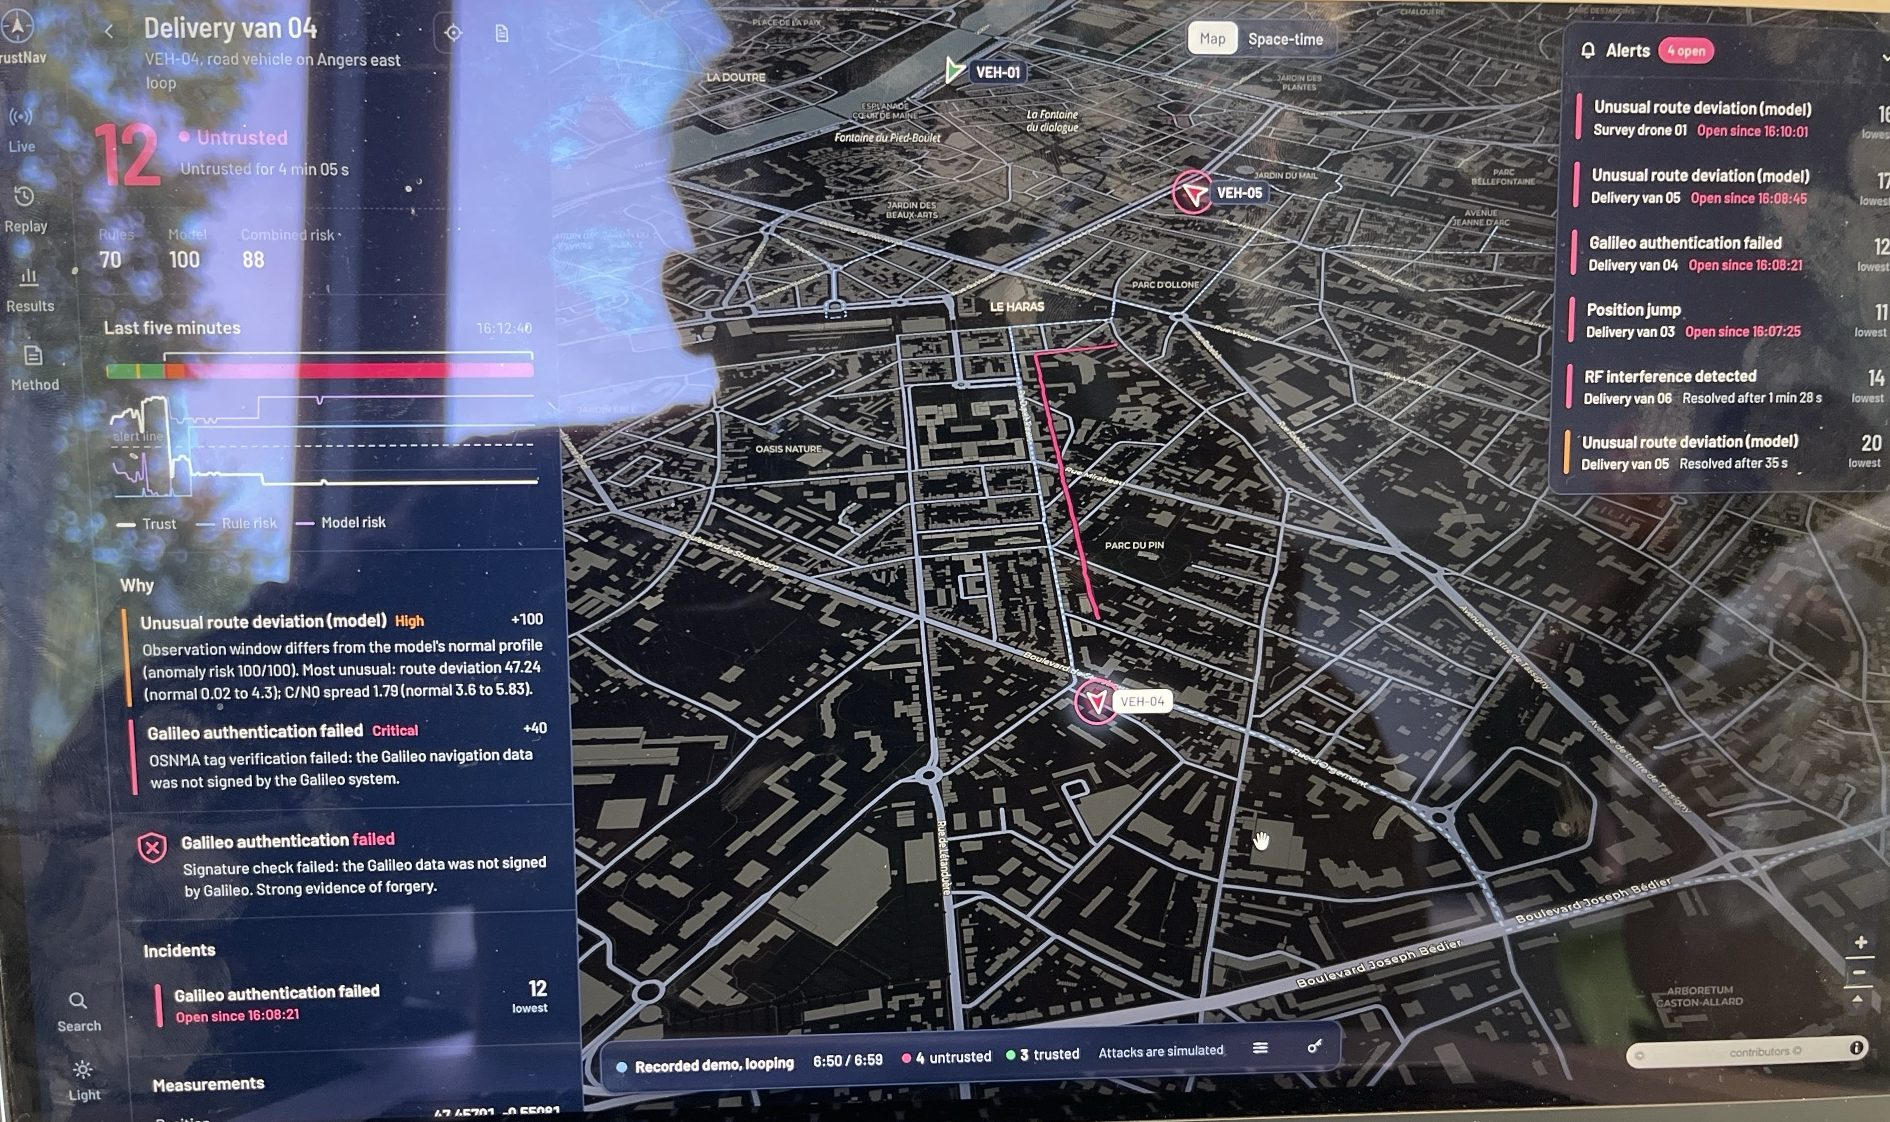
\includegraphics[width=\columnwidth]{figures/console-photo.jpg}
\caption{The deployed console: Delivery van 04 under a Galileo forgery attack, untrusted for four minutes, with the forged track in pink over the real streets of Angers. The panel lists the evidence (route deviation flagged by the model, OSNMA failure) with the measured values and thresholds.}
\label{fig:console}
\end{figure}

Every decision is explained twice: as the evidence lines the engine produced (``Position moved 8\,003\,m in 1\,s (limit 250\,m)''), and as a verdict in everyday words derived from the evidence codes alone, so that it works unchanged on a real receiver (``The receiver places the van 8.0\,km from the road it is actually on. A transmitter is imitating the satellites. \sys\ has stopped passing this position on and is tracking the van by its odometer along its route''). On the map a refused fix is drawn hollow, a shield marks the protected estimate, and a dashed line between them carries the size of the lie (Fig.~\ref{fig:map}).

\begin{figure}[t]
\centering
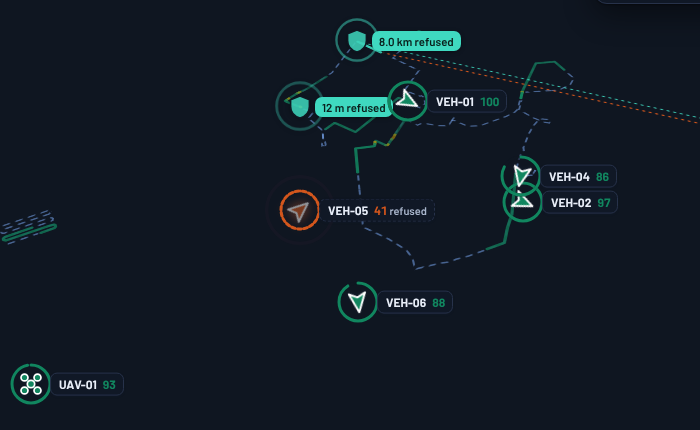
\includegraphics[width=\columnwidth]{figures/map-protection.png}
\caption{The response layer on the map: hollow markers are refused fixes, shields are the protected estimates, dashed lines the lies (``8.0 km refused''). Street tiles are omitted in this test render.}
\label{fig:map}
\end{figure}

\section{Evaluation}\label{sec:eval}

\subsection{Data and protocol}
No public dataset provides labelled per-second receiver observables for fleets with routes and odometers, and transmitting attacks is illegal, so a deterministic, seeded simulator produces the observations a receiver would report. Road routes are real Angers street geometry routed with OSRM on OpenStreetMap data; drone missions are generated lawnmower surveys. Normal behaviour includes the things that cause false alarms in practice: traffic stops, cornering and urban-canyon segments where buildings cut satellites and raise residuals. Attack overlays, each labelled per observation, are: an 8\,km teleport by a GPS-only spoofer (OSNMA becomes unavailable); a gradual drift under 1\,m/s with the spoofer's power visible in C/N$_0$; a spoofer onset in which C/N$_0$ jumps and becomes unnaturally uniform while the position barely moves; a relay-style \emph{stealth drift} in which the signal stays clean and OSNMA still verifies; an OSNMA forgery; broadband jamming with loss and recovery of the fix; and a drone pushed off its survey line.

Routes are assigned one role each and never shared: five road loops and two drone areas for \emph{training} (normal runs only, 10\,785 observations for fitting and 5\,630 for calibration), two loops and one drone area for \emph{validation} (fusion weights only), and two loops and one drone area for the \emph{held-out} catalogue that produces every reported number: ten scenarios, 3\,800 one-second observations, 1\,550 of them under attack. An observation is the evaluation unit; an alert is a combined risk of 50 or more.

\subsection{Detection}
Table~\ref{tab:detect} compares the three ways to decide. Rules never raise a false alarm but miss slow attacks; the model catches subtle change but is noisier; combined, each covers the other's blind spot. Table~\ref{tab:scen} gives, per scenario, the time from attack start to the first alert. All seven attack types are caught; the stealth drift, invisible to every rule and to OSNMA, is caught by the model after 42\,s at roughly 12\,m off the road, where the fixed 150\,m route rule alone would need about 3.5\,min.

\begin{table}[t]
\caption{Detection on the held-out catalogue (3\,800 observations)}
\label{tab:detect}
\centering
\begin{tabular}{@{}lrrr@{}}
\toprule
 & Rules only & Model only & \textbf{Combined} \\
\midrule
Precision & 100.0\,\% & 97.9\,\% & \textbf{99.3\,\%} \\
Recall & 27.9\,\% & 90.1\,\% & \textbf{96.1\,\%} \\
F$_1$ & 0.437 & 0.939 & \textbf{0.977} \\
False-alarm rate & 0.00\,\% & 1.33\,\% & \textbf{0.44\,\%} \\
ROC AUC & 0.857 & 0.937 & \textbf{0.990} \\
Mean time to detect & 9.0\,s & 6.6\,s & \textbf{6.7\,s} \\
\midrule
True positives & 433 & 1\,397 & 1\,489 \\
False positives & 0 & 30 & 10 \\
False negatives & 1\,117 & 153 & 61 \\
True negatives & 2\,250 & 2\,220 & 2\,240 \\
\bottomrule
\end{tabular}
\end{table}

\begin{table}[t]
\caption{Time from attack start to first alert, per held-out scenario}
\label{tab:scen}
\centering
\begin{tabular}{@{}lrrrr@{}}
\toprule
Scenario & Rules & Model & \textbf{Comb.} & FA \\
\midrule
Normal drive, centre loop (420 obs.) & -- & -- & -- & 0 \\
Normal drive, east loop (420) & -- & -- & -- & 2 \\
Teleport spoof, 8\,km jump & 0\,s & 1\,s & \textbf{0\,s} & 0 \\
Gradual drift spoof & missed & 1\,s & \textbf{1\,s} & 0 \\
Signal anomaly (spoofer onset) & missed & 1\,s & \textbf{1\,s} & 0 \\
Stealth drift (OSNMA verified) & missed & 40\,s & \textbf{42\,s} & 0 \\
OSNMA forgery & 15\,s & 1\,s & \textbf{1\,s} & 0 \\
Jamming with recovery & 12\,s & 1\,s & \textbf{1\,s} & 6 \\
Drone survey, normal (360) & -- & -- & -- & 2 \\
Drone spoofed off mission & missed & 1\,s & \textbf{1\,s} & 0 \\
\bottomrule
\end{tabular}
\\[2pt]{\footnotesize FA: false alerts (clean seconds flagged) in that run.}
\end{table}

\subsection{What the response layer prevents}
Because the simulator knows the true position, we can measure, during each attack, the worst position an ordinary fleet screen would have shown (the raw fix) against the worst position the response layer handed downstream (Table~\ref{tab:prot}). Across the spoofing scenarios the worst reported error is 8\,003\,m and the worst protected error 29\,m; during the 100\,s jamming outage an ordinary screen is blank while the estimate stays within 2\,m. Holds begin in the same second or the second after the alert, and persist for the attack. The cost is small: a hold adds a few metres of odometer error even when the attack did not move the position (signal anomaly, 20.8\,m), and holds outside any attack, from a brief dip on a normal run or the seconds after an attack ends before the fix rejoins the estimate, total 26\,s over the whole catalogue.

\begin{table}[t]
\caption{Worst position error during the attack, against ground truth}
\label{tab:prot}
\centering
\begin{tabular}{@{}lrrr@{}}
\toprule
Scenario & Raw fix & \textbf{Protected} & Hold after \\
\midrule
Teleport spoof & 8\,003\,m & \textbf{3.8\,m} & 0\,s \\
Gradual drift spoof & 211\,m & \textbf{16.3\,m} & 1\,s \\
Signal anomaly & 6.8\,m & \textbf{20.8\,m} & 1\,s \\
Stealth drift & 179\,m & \textbf{20.1\,m} & 42\,s \\
OSNMA forgery & 130\,m & \textbf{15.4\,m} & 1\,s \\
Jamming (100\,s no fix) & blank & \textbf{1.8\,m} & 1\,s \\
Drone spoofed off mission & 257\,m & \textbf{28.8\,m} & 1\,s \\
\bottomrule
\end{tabular}
\end{table}

\section{Discussion and Limitations}\label{sec:discussion}
The numbers above are an upper bound. One simulator produces every split, so the model's notion of ``normal'' is the simulator's; the attack overlays are textbook versions, and a careful adversary who matches C/N$_0$ spread and clock behaviour would be harder to detect. Route deviation assumes an assigned route, which holds for delivery fleets and survey drones but not for a driver who changes route. OSNMA status is simulated, and a long attack contributes many correlated observations, so per-observation scores are not per-attack accuracy. The receiver dependence reported by Kriezis \emph{et al.} \cite{kriezis2025} is the central risk for transfer to hardware: thresholds and the learned normal must be re-calibrated on the receiver actually used.

The validation plan follows from this. First, a real receive-only GNSS receiver (u-blox M8/M9 class, about \texteuro60; or a ZED-F9P with a multi-band antenna, about \texteuro250, whose recent firmware supports OSNMA) is connected through the existing adapter and the engine runs with rules only. Second, normal drives around Angers are recorded and the thresholds and model are re-calibrated on them, reporting the false-alarm rate before and after. Third, public attack recordings, the FGI Jammertest 2023 I/Q captures \cite{fgi2023} and TEXBAT \cite{texbat}, are replayed through a software receiver into the same pipeline to obtain real attack detection figures without transmitting anything. Beyond that, a vehicle's odometer or OBD-II speed as the inertial input, a second cheap receiver on the same vehicle to catch synchronous spoofing (two real antennas see different satellites, a single spoofer makes both report the same position), real OSNMA from raw Galileo pages, and map matching for vehicles without an assigned route are the next layers of evidence.

\section{Safety, Legal and Ethical Considerations}\label{sec:ethics}
No signal is transmitted at any point in this work: every attack exists as software. Transmitting on the GNSS bands is illegal in France and harms every receiver nearby \cite{anfr2024}; real attack testing will use recordings or a shielded laboratory with a licence. The Phase~2 hardware is receive-only. The demo involves no personal data, but a real deployment tracks vehicles and therefore their drivers, so purpose limitation, retention (the demo database prunes live frames after three days), access control and transparency towards drivers apply under the GDPR. The system's own security (hashed tokens, rate-limited passcode, read-only public access) is part of the design. The trust score is a research indicator, not a certified integrity figure, and \sys\ is not for aviation, maritime or other safety-critical use.

\section{Conclusion}
\sys\ shows that a software layer beside an ordinary receiver can give a fleet operator what neither receiver flags nor fixed probes provide: a per-second, explained trust score for every platform, and a response that keeps a false position from reaching the systems that act on it. On held-out synthetic scenarios the hybrid of explainable rules, an unsupervised model and Galileo authentication reaches an F$_1$ of 0.977 with 0.44\,\% false alarms and catches a relay-style drift that defeats authentication, while the response layer bounds the operator-visible error to tens of metres instead of kilometres. The decisive next step is the one the simulator cannot provide: real receiver data, which the adapter, the calibration plan and the public attack recordings are ready for.

\balance
\section*{Acknowledgment}
The authors thank Sofiane Hamrioui, ESAIP Angers, for supervising this project. Map data \copyright\ OpenStreetMap contributors; basemaps \copyright\ CARTO; road routes computed with OSRM.

\begin{thebibliography}{00}
\bibitem{anfr2024} ANFR and DGITM, ``Guide: le brouillage des syst\`emes de radionavigation par satellite,'' Feb. 2024. [Online]. Available: \url{https://anfr.fr/fileadmin/mediatheque/documents/brouillage/ANFR-DGITM_-_Guide_Brouillage_VD_-_2024.pdf}
\bibitem{rntf2017} Resilient Navigation and Timing Foundation, ``GPS jammer delays flights in France,'' Sep. 2017. [Online]. Available: \url{https://rntfnd.org/2017/09/15/gps-jammer-delays-flights-in-france/}
\bibitem{transinfo2023} trans.info, ``GPS jammer that brought disruption to Lyon airport,'' Jul. 2023. [Online]. Available: \url{https://trans.info/en/gps-jammer-that-brought-disruption-to-lyon-airport-353510}
\bibitem{insidegnss2013} Inside GNSS, ``FCC fines operator of GPS jammer that affected Newark airport GBAS,'' Aug. 2013. [Online]. Available: \url{https://insidegnss.com/fcc-fines-operator-of-gps-jammer-that-affected-newark-airport-gbas/}
\bibitem{eucouncil2025} Council of the European Union, ``Note on GNSS interference in the Baltic region,'' ST 9188/25, May 2025. [Online]. Available: \url{https://data.consilium.europa.eu/doc/document/ST-9188-2025-INIT/en/pdf}
\bibitem{opsgroup2024} OpsGroup, ``GPS spoofing: final report of the GPS Spoofing WorkGroup,'' Sep. 2024. [Online]. Available: \url{https://ops.group/blog/gps-spoofing-final-report/}
\bibitem{geotab2025} Geotab, ``Combating GPS jammers,'' Jul. 2025. [Online]. Available: \url{https://www.geotab.com/blog/combating-gps-jammers/}
\bibitem{ublox2024} u-blox, ``ZED-F9P FW 1.00 HPG 1.50 release note,'' UBXDOC-963802114-12826, 2024. [Online]. Available: \url{https://content.u-blox.com/sites/default/files/documents/ZED-F9P_FW100HPG150_RN_UBXDOC-963802114-12826.pdf}
\bibitem{ublox_jammertest} u-blox, ``GNSS jamming and spoofing detection at Jammertest 2025,'' 2025. [Online]. Available: \url{https://www.u-blox.com/en/blogs/tech/gnss-jamming-spoofing-detection-jammertest-2025-andoya}
\bibitem{septentrio2025} Septentrio, ``AIM+ spoofing protection,'' 2025. [Online]. Available: \url{https://www.septentrio.com/en/learn-more/advanced-positioning-technology/aim-spoofing-protection}
\bibitem{gpspatron} GPSPatron, ``Detecting GNSS threats'' and ``GP-Probe TGE2 datasheet,'' 2024. [Online]. Available: \url{https://gpspatron.com/detecting-gnss-threats/}
\bibitem{gpsdome2} GPS World, ``infiniDome releases GPSdome 2 dual-band anti-jamming technology,'' Oct. 2022. [Online]. Available: \url{https://www.gpsworld.com/infinidome-releases-gpsdome-2-dual-band-anti-jamming-technology/}
\bibitem{gpsjam} J. Wiseman, ``GPSJam: FAQ.'' [Online]. Available: \url{https://gpsjam.org/faq/}
\bibitem{fr24} Flightradar24, ``GPS jamming map.'' [Online]. Available: \url{https://www.flightradar24.com/data/gps-jamming}
\bibitem{euspa2025} EUSPA, ``Galileo OSNMA service now available to users,'' Jul. 2025. [Online]. Available: \url{https://www.euspa.europa.eu/newsroom-events/news/testing-operations-galileo-osnma-service-now-available-users}
\bibitem{gsc_faq} European GNSS Service Centre, ``OSNMA frequently asked questions.'' [Online]. Available: \url{https://www.gsc-europa.eu/node/7832}
\bibitem{wang2025} H. Wang, Y. Zhang, Y. Tan, J. He, S. Zhao, N. Xi, and Y. Shen, ``Practical spoofing attacks against Galileo OSNMA with time-synchronization manipulation,'' arXiv:2501.09246, 2025.
\bibitem{texbat} T. E. Humphreys, J. A. Bhatti, D. P. Shepard, and K. D. Wesson, ``The Texas Spoofing Test Battery: Toward a standard for evaluating GPS signal authentication techniques,'' in \emph{Proc. ION GNSS}, Nashville, TN, USA, 2012.
\bibitem{tang2025} Y. Tang and Q. Qin, ``GNSS spoofing detection based on LSTM-TNN-CVAE network,'' in \emph{Proc. APSIPA ASC}, 2025, pp. 1830--1834.
\bibitem{iqbal2025} A. Iqbal, M. N. Aman, and B. Sikdar, ``A time-series based convolutional VAE for spoof detection in commercial GPS receivers,'' 2025. [Online]. Available: \url{https://www.ece.nus.edu.sg/stfpage/bsikdar/papers/ccnc_25b.pdf}
\bibitem{li2025} J. Li \emph{et al.}, ``Performance testing and analysis of a new GNSS spoofing detection method in different spoofing scenarios,'' \emph{IEEE Access}, vol. 13, pp. 54779--54793, 2025, doi: 10.1109/ACCESS.2025.3553475.
\bibitem{bhuiyan2026} M. Z. H. Bhuiyan \emph{et al.}, ``Implementation and performance analysis of a chi-square test based GNSS signal anomaly detection,'' \emph{GPS Solutions}, vol. 30, art. 154, 2026, doi: 10.1007/s10291-026-02102-z.
\bibitem{kriezis2025} A. Kriezis, Y.-H. Chen, D. Akos, S. Lo, and T. Walter, ``Real-world spoofing detection and characterization using low-cost receivers,'' in \emph{Proc. ION ITM}, 2025. [Online]. Available: \url{https://web.stanford.edu/group/scpnt/gpslab/pubs/papers/Kreizis_ION_ITM_2025_Real_World_Spoofing_Detection.pdf}
\bibitem{liu2008} F. T. Liu, K. M. Ting, and Z.-H. Zhou, ``Isolation forest,'' in \emph{Proc. IEEE Int. Conf. Data Mining}, 2008, pp. 413--422.
\bibitem{sklearn} F. Pedregosa \emph{et al.}, ``Scikit-learn: Machine learning in Python,'' \emph{J. Mach. Learn. Res.}, vol. 12, pp. 2825--2830, 2011.
\bibitem{fgi2023} Finnish Geospatial Research Institute, ``FGI Jammer Test 2023 repository,'' 2024. [Online]. Available: \url{https://etsin.fairdata.fi/dataset/2eee8cfd-db00-4e46-bd62-d7632c09c700}
\end{thebibliography}

\end{document}
